\chapter{Diseño}\label{cap:disenio}

En este capitulo se documentara como se desarrollo el diseño de la arquitectura del proyecto, para ello se expondrá el modo en que trabaja \jd y además se mostrara la estructura de clases que se eligió para el sistema para que pueda cumplir con los requisitos expuestos en el Capitulo \ref{capitulo:especificacion}.





\section{Visión general}

Para diseñar \jj como ya se menciono se tomo como base a el patrón de desarrollo DAO que se explico en la sección \fullref{jdbgm:dao}, siguiendo la idea de este patrón \jj debe manejar todas las consultas echas a el motor por lo que la aplicación solo se deberá comunicar con \jj para acceder a el motor de base de datos, se puede observar esquemáticamente esta idea en la figura \figpage{fig:jdbgm:overview} en la que podemos observar que la idea es que la aplicación utilice el formato que estamos proponiendo para trabajar con las sentencias SQL, estas serán interpretadas por \jj y convertidas a una cadena de texto la cual es entendible por \jd y este se comunicara directamente con el DBMS y pondrá a disposición de \jj el resultado que dependiendo de la consulta puede ser un objeto del tipo \verb=ResultSet= o un tipo \verb=integer=. 

\begin{figure}
  \centering
    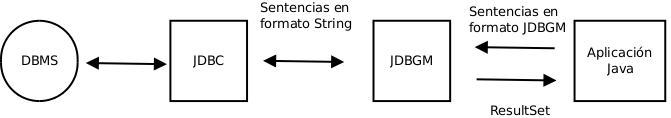
\includegraphics[width=0.85\textwidth]{figuras/jdbgm-overview.png}
  \caption{JDBGM dentro de una aplicación}
  \label{fig:jdbgm:overview}
\end{figure}

Así que \jj debe ser capaz de hacer dos tareas independientes pero relacionadas, en primer lugar debe proveer el almacenamiento de las sentencias de modo que puedan ser traducidas luego a el dialecto que corresponda y en segundo lugar proveer los métodos necesarios para comunicarse con el motor mediante \jd, podemos observar esquemáticamente la situación en la figura \figpage{fig:jdbgm:closerlook} que nos muestra la idea de independencia existente entre los dos módulos principales que se están exponiendo, el manejador de sentencias es totalmente independiente de la capa intermedia pues de lo que esta encargado es de proveer los métodos necesarios para ``armar las sentencias'' y traducirlas cuando sea requerido a el dialecto correspondiente, esta traducción lo que hace es convertir la sentencia almacenada a una cadena de texto la cual es entendible por \jd por lo que se podría obviar la capa intermedia que hace transparente su uso y usarlo directamente. En cambio la capa intermedia dependerá de el manejador de sentencias para poder proveer la independencia de dialectos que se quiere lograr y además este solo recibirá las sentencias compatibles con el formato propuesto por \jj por lo que a continuación se procederá a explicar la estructura propuesta para este manejador para que después se pueda explicar correctamente el funcionamiento de la capa intermedia.

\begin{figure}
  \centering
    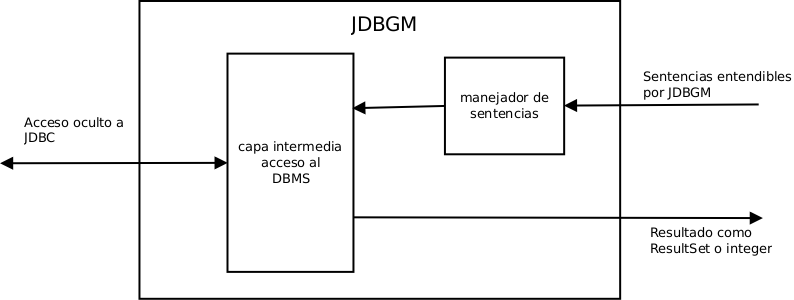
\includegraphics[width=0.85\textwidth]{figuras/jdbgm-closerlook.png}
  \caption{Vista abstracta del funcionamiento de JDBGM}
  \label{fig:jdbgm:closerlook}
\end{figure}

\section{Manejador de sentencias}
Como ya se dijo el manejador de sentencias debe ser capaz de almacenar las sentencias de forma desglosada así que pasemos a ver que se quiere lograr. Como una primer solución podemos pensar que una sentencia como la siguiente ``\verb=nombre_comando parametro opcion1 parametro1 opcion2 parametro2='' que se podría corresponder con la siguiente consulta ``\verb|SELECT * FROM table WHERE table.id=1|'', salvando ciertas reglas de construcción que en este momento no vienen al caso, puede ser almacenado en una clase que se corresponda con el siguiente esquema:

\begin{lstlisting}[title=Pseudocódigo de la estructura de dato que contiene la sentencia]
class Sentencia{
	nombre_comando;
	parametro;
	set_opcion1(parametro1);
	set_opcion2(parametro2);
	devolver_sentencia();
}
\end{lstlisting}
Como se ve es una idea bastante sencilla en la que la clase identificara la sentencia y sus opciones correspondientes serán nombres de atributos pues en definitiva lo que nos interesa de estas opciones son los valores que toman o si están presentes o no en la sentencia que se esta armando. Como clase de POO también debe ofrecer métodos para almacenar los valores que tomaran las opciones y es aquí donde empiezan a jugar las reglas dispuestas en el dialecto genérico que fue especificado en el capitulo \ref{capitulo:especificacion}, puesto que las opciones ofrecidas por cada sentencia no pueden ser libremente usadas es necesario que estos métodos restrinjan el modo en que se pueden usar ya sea limitando las posibilidades de el/los métodos o bien usando excepciones para detener la ejecución del programa, una explicación mas detallada del manejo de excepciones se vera en las secciones siguientes, cuando alguna acción ilegal sobre las sentencias ocurra.

Con esto ya se tiene una idea genérica de las clases que se quiere representen a las sentencias y teniendo en cuenta que cada una de estas clases representa a una sentencia diferente con un comportamiento diferente pero con similitudes es necesario recalcar que estas diferentes clases deben presentar las mismas similitudes, por ejemplo supóngase que los objetos \verb|select| y \verb|create| representan las sentencias SQL del mismo nombre las cuales precisan que se les asigne el nombre de la tabla sobre la que se esta trabajando entonces lo correcto sera que ambos objetos tengan un método de igual nombre y comportamiento igual como por ejemplo \verb=select.set_table_name("name_1")= y \verb=create.set_table_name("name_2")=. Es muy importante tener en cuenta esto puesto que facilitara el aprendizaje del uso de la API del manejador de sentencias que se esta proponiendo y además hará el uso de la misma mucho mas natural, con respecto a SQL. Antes de empezar a hablar de lleno de la arquitectura propuesta para el manejador de sentencia es necesario nombrar al paquete \cc de el cual se tomaron algunas ideas.

\subsection{El paquete \cc}
Este paquete que puede ser encontrado en \href{http://sourceforge.net}{SourceForge} en la siguiente dirección \url{http://sourceforge.net/projects/crossdb/} intenta solucionar el mismo problema que el manejador de sentencias aquí presentado tal como se puede observar en la pagina del proyecto que se resume en la siguiente oración:

\begin{center}
``To provide cross database tools for manipulating all major databases without having to worry about each vendors specific implementation.''
\end{center} 

Esta librería  usa la misma idea de ir generando bajo demanda las sentencias por lo que se la estudio y se llego a la conclusión de que podía servir como base para el manejador que se quiere implementar en este proyecto. Algunas consideraciones antes de avanzar:
\begin{itemize}
\item El paquete se distribuye bajo Apache Software License 1.1 por lo que no hay inconvenientes en reusar el código escrito, siempre y cuando se respeten las condiciones impuestas. Además esta licencia es compatible con GPL.
\item La ultima actualización del proyecto data el 23-08-2005 (la ultima modificación registrada en el repositorio svn) por lo que aparentemente el proyecto quedo en un punto muerto y en una versión beta básica según se puede ver al revisar el código.
\item Carece de una buena documentación pero el código es bastante entendible y mas aun después de venir estudiando una solución similar a la propuesta por \cc


\end{itemize}
Se puede resumir la estructura usada por esta librería en el gráfico \fullref{fig:crossdb:base-idea} que nos muestra que por cada sentencia existe una Interfaz \verb=Statement= que define el comportamiento de la misma, luego para esta interfaz base existe una implementación por defecto \verb=DefaultStatement= que implementa las funciones que son comunes a toda implementación que se pueda realizar de dicha interfaz, recordando que al trabajar con dialectos estamos trabajando con variaciones de un lenguaje base, y por cada una de estas implementaciones por defecto existe una implementación especifica \verb=SpecificStatement= que contempla las particularidades de un motor en particular sobre dicha sentencia. En la misma figura podemos observar como se conforma dicha arquitectura para la sentencia \verb=SELECT= con la clases \verb=SelectQuery= siendo la interfaz base, \verb=DefaultSelectQuery= siendo la implementación por defecto de dicha interfaz y \verb=OracleSelectQuery= una implementación especifica para el dialecto usado por Oracle.


%\begin{figure}
%  \centering
%    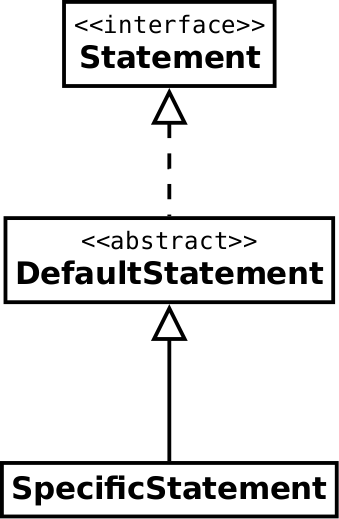
\includegraphics[width=0.2\textwidth]{figuras/crossdb-base-idea.png}
%  \caption{Vista abstracta de la arquitectura de crossdb}
%  \label{fig:crossdb:base-idea}
%\end{figure}
\begin{figure}
  \centering
  \subfloat[Idea base]{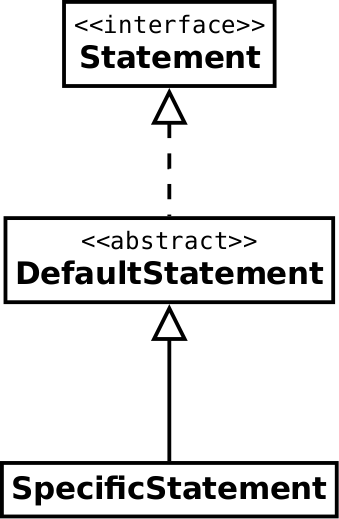
\includegraphics[width=0.2\textwidth]{figuras/crossdb-base-idea.png}} \label{fig:subfig:crossdb:base-idea}
  \qquad 
  \subfloat[Ejemplo con Select]{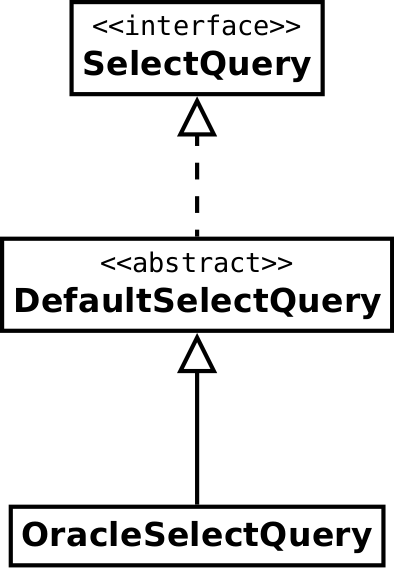
\includegraphics[width=0.2\textwidth]{figuras/crossdb-base-idea-select.png}} \label{fig:subfig:crossdb:base-idea-select}
  \caption{Vista abstracta de la arquitectura de crossdb}
  \label{fig:crossdb:base-idea}
\end{figure}

Además de las clases a las que se hizo referencia \cc usa otras auxiliares, como \verb=Column= que contiene los datos necesarios para especificar una columna o \verb=WhereClause= que representa una clausula \verb=WHERE=, necesarias para poder almacenar adecuadamente los datos para las sentencias que se están armando. También se implementa la idea del patrón Factory pero de una manera muy básica. Terminado de presentar ligeramente este paquete sobre el cual se baso el diseño propuesto en este trabajo se pasara a exponer la arquitectura usada por el manejador de sentencias y su relación con las ideas tomadas de \cc.

\subsection{Diseño básico de el Manejador}
%Para la implementación de las especificaciones declaradas anteriormente nos encontramos con que existen algunas similitudes entre las diferentes clases definidas anteriormente, atendiendo a que cada clase representa a una de las sentencias SQL que se incluyeron en el proyecto y cada clase esta compuesta por:
Recordando lo expuesto en la sección anterior sobre las clases que representan las sentencias podemos resumir su contenido de manera muy genérica de la siguiente manera:

\begin{itemize}
\item Variables que almacenaran los datos necesarios para la construcción de los métodos, aunque también puede ser necesario el uso de clases auxiliares dependiendo de la complejidad de la clase.

\item Métodos para inicializar la clase y agregar (lo que comúnmente se dice \textit{setear}), es decir poblarla con los datos necesarios para su construcción.

\item Un método para armar la sentencia.

\end{itemize}

La estructura de cada una de estas clases puede ser implementada directamente desde las restricciones impuestas en la sección \fullref{seccion:especificacion:dialectos} pero siguiendo ciertos lineamientos que veremos a continuación.

En primer lugar se tiene que tener en cuenta la arquitectura general de el manejador para ello hay que observar lo siguiente: se puede hacer una distinción en como es que responde el motor de base de datos a las sentencias, o mas bien como responde JDBC, que es el "interlocutor" cuando procesa determinada sentencia SQL. Por un lado están aquellos que solo necesitan reportar la cantidad de filas afectadas por la sentencia después están aquellos que necesitan devolver información después de ejecutada la sentencia, estas ultimas sentencias son precisamente las que realizan consultas sobre la base de datos siendo las sentencias \verb=SELECT= las únicas que hacen esto. Por otro lado las sentencias \verb=UPDATE=, \verb=INSERT= y \verb=DELETE= solo precisan reportar la cantidad de filas que fueron afectadas por la consulta, en cambio las sentencias \verb=ALTER TABLE= y \verb=CREATE TABLE= que sirven para modificar las tablas (son parte del DDL de SQL) no afectan directamente a las filas de la misma pero por convención se tomo que \jd devuelva 0 como numero de columnas afectadas por lo que en este caso se las agrupara en el mismo conjunto. Entonces para que \jj pueda hacer distinción de estos dos tipos de consultas se utilizaron dos interfaces las cuales pueden ser tomadas como tipos genéricos, la \figpage{fig:crossdb-base} muestra estas interfaces y sus hijas.

\begin{figure}
  \centering
    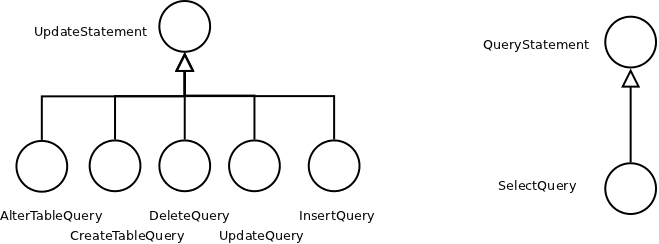
\includegraphics[width=0.65\textwidth]{figuras/crossdb-base.png}
  \caption{Interfaces base para los tipos de sentencia}
  \label{fig:crossdb-base}
\end{figure}

De este modo se utilizan las interfaces \verb=UpdateStatement= y \verb=QueryStatement= como un tipo genérico para identificar las sentencias que no realizan consultas de aquellas que si, es decir si en la firma de cualquier método se declara algo similar a lo siguiente \verb=metodo_a(UpdateStatement statement)= el parámetro \verb=statement= podrá ser cualquier clase que sea heredera directa o indirectamente de la interfase \verb=UpdateStatement= y no podrá tomar ninguna heredera de la clase \verb=QueryStatement=, en este caso la herencia de la interfaz base sera indirecta como se aclarara a continuación y además cabe aclarar que este es el primer cambio que se agrego a la estructura que proponía \cc.

\begin{figure}
  \centering
    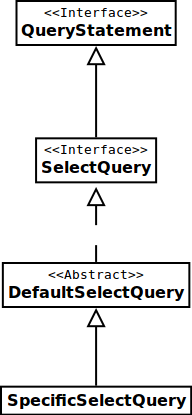
\includegraphics[width=0.65\textwidth]{figuras/crossdb-query.png}
  \caption{Diagrama de clases para la sentencia SELECT}
  \label{fig:query-base}
\end{figure}

En la \figpage{fig:query-base} tenemos una vista completa de como se debe componer la estructura de clases para el tipo base \verb=QueryStatement=, que es la mas simple pues solo tiene una clase hija, la única que sirve para hacer consultas sobre la base de datos la sentencia \verb=SELECT=. Como ya se dijo la primer interfase sirve para distinguir a nivel genérico el tipo de sentencia SQL que se esta tratando, la interfase hija directa de \verb=QueryStatement= si ya define un comportamiento especifico para las funciones de las sentencias \verb=SELECT=. La clase abstracta \verb=DefaultSelectQuery= brinda una implementación base para los métodos definidos en \verb=SelectQuery=, para comprender por que se debe hacer esto es necesario recordar que la clase que represente una sentencia contiene toda la información necesaria para generar una sentencia valida y esta información es la misma que se precisa para cualquier sentencia SQL de un dialecto en concreto (además ya se definió una sintaxis que es totalmente soportada) la diferencia esta en el modo que se escriben las sentencias, la sintaxis, por ello el único método que deberá ser especifico a un \dd será aquel que esta encargado de armar la sentencia. Después de la clase abstracta si por fin tenemos implementaciones especificas para cada uno de los motores, estas son la clase \verb=SpecificSelectQuery=de las que se hablaba en la \figpage{fig:crossdb:base-idea}, la idea es que de estas clases hayan tantas como motores estén soportados por el proyecto.

\begin{figure}
  \centering
    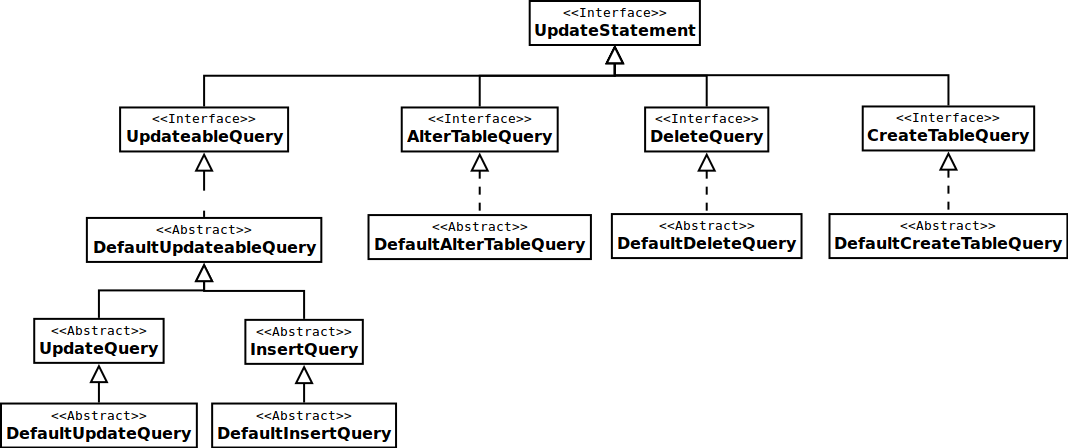
\includegraphics[width=\textwidth]{figuras/crossdb-update.png}
  \caption{Estructura de las otras sentencias}
  \label{fig:update}
\end{figure}

En la \figpage{fig:update} tenemos una descripción de como se deben estructurar los tipos de la interfaz base \verb=UpdateStatement=, esta es algo mas elaborada pero como antes la primer interfaz, funciona como tipo genérico, en las clases hijas de esta vemos algo parecido al caso de \verb=QueryStatement= salvo por la interfaz \verb=UpdateableQuery= que agrupa comportamiento común a \verb=Updatequery= e \verb=InsertQuery=, también se brinda un comportamiento predeterminado para esta mediante \verb=DefaultUpdateStatement= pero el cual al brindar una implementación base tiene que ser a la fuerza una clase abstracta\footnote{Una clase abstracta se puede ver como una interfaz que fuerza la implementación de parte de su comportamiento} así que las clases que definen el comportamiento especifico de \verb=UpdateQuery= e \verb=InsertQuery= son clases abstractas y no interfaces, pero el resultado es el mismo. Y finalmente para cada una de las interfaces que definen(o representan) a las sentencias tenemos una implementación por defecto en las clases cuyo nombre empieza por \verb=Default= de las cuales deberán heredar cada una de las implementaciones especificas, en la figura \ref{fig:update} no se las representa puesto que seria demasiado extenso.

Después de analizar el dialecto genérico que se definió en la sección \fullref{seccion:especificacion:dialectos} y de definir la estructura de las clases para el manejador se buscaron aquellos atributos de las clases (extraídos de las sentencias que representan) que por su complejidad ameritaban convertirse en una clase por si mismas, tal es el caso de una columna que en si es una entidad distinguible y lo suficientemente compleja como ejemplo podemos notar que una columna posee nombre, tipo de dato que almacena y muchas otras restricciones que pueden ser encontradas en el capitulo \ref{cap:disenio} en la sección que se refiere a la sentencia \verb=CREATE TABLE=. A continuación se listan y explican las clases auxiliares que se encontraron. 

%un análisis mas detallado de como se componen las interfaces finales y las clases que las implementan además de una vista a su implementación y las clases que sirven como componente de las principales.
\subsection{Clases Auxiliares} \label{seccion:disenio:clases-auxiliares}
Como ya se denoto para un adecuado y consistente funcionamiento de el manejador de sentencias es necesario crear algunas clases extras que brindan funcionalidades comunes a varias clases o bien funcionalidades extras no propias de dichas clases que ayudaran a formar las similitudes entre las diferentes clases que representan a las sentencias, a continuación un listado de estas:

\begin{itemize}
\item \verb=Column=
\item \verb=DataTypes=
\item \verb=Formater=(No usado - revisar)
\item \verb=Functions= (no decidido por completo)
\item \verb=Join=
\item \verb=SpecificSQLFactory=
\item \verb=SQLFactory=
\item \verb=SQLFormat, SQLDateTimeFormat, SQLTimeFormat=
\item \verb=WhereClause, WhereCondition, WhereFrame=
\end{itemize}
A continuación una descripción de ellas

\subsubsection{La clase Column}
Representa una columna de una tabla para ello posee atributos tales como nombre de columna, banderas que indican si es clave primaria o foranea y todos los demás atributos que sirven para definir la columna en una sentencia \verb=CREATE TABLE=. Entre sus métodos no se incluye ninguno que sirva para convertir la columna en una cadena  de texto que sirva para definirla en una sentencia SQL pues a pesar de que la sintaxis de la definición de columna no varia, salvo por los tipos de datos, si varia el uso sobre ella pues la sentencia \verb=ALTER TABLE= también puede definir columnas en su sintaxis pero con ciertas restricciones como se ve en la sección \ref{sec:altertable} y para evitar confusiones cada clase (clase que represente una sentencia) que haga uso de un objeto columna deberá implementar las restricciones sobre la construcción de la sentencia ignorando los atributos que no use.

Además de esto la columna también posee un atributo para almacenar un valor para la columna de modo que la clase no solo sirva para definir una columna si no también como contenedor del valor, del tipo y del nombre  de la columna para usarlo luego con otras sentencias que no necesiten definir columnas si no ingresarles datos como es el caso de \verb=INSERT=. Haciendo esto se evita crear otra clase que solo sirva de contenedor para el valor de una columna y por lo tanto hay menos clases para recordar. 



\begin{enumerate}
\item \verb=Column= 
\item \verb=DataTypes= Es una clase abstracta que define el comportamiento de las clases que serán encargadas de mapear los tipos de datos genéricos usados en \cc a los tipos de datos concretos para cada motor, la clase define un solo método \verb=getAsString(Column col)= que a partir de un objeto \verb=Column= tomado como parámetro devuelve una cadena de texto que contiene el tipo de datos especifico. Aparte se tiene un método abstracto que tiene por objetivo concreto mapear el tipo de dato genérico con el tipo especifico.  

\item \verb=Formatter=

\item \verb=WhereCondition= Es una clase muy simple que tiene por objetivo la representación de las condiciones $ x = y $ que se usan dentro de una cláusula WHERE. La clase puede contener los nombres de las tablas a comparar, si es que se comparan valores de mas de una tabla, los nombres de los campos a comparar y (de haber) algún valor contra el que comparar.

\item \verb=WhereClause=  Representa una cláusula \verb=WHERE= como por ejemplo \verb|WHERE x = y | , la cláusula where esta formada por diferentes condiciones del tipo \verb=WhereCondition= e incluir cláusulas \verb=WhereClause= anidadas como por ejemplo \verb|WHERE (x = y AND (x=z OR x=b))|. Entonces cada conjunto de paréntesis puede ser visto como una cláusula \verb=WHERE=, y básicamente podemos ver a \verb=WhereClause= como una lista de condiciones y/o cláusulas \verb=WHERE=.

\item \verb=Join= Básicamente representa las condiciones de \verb=JOIN= para las sentencias \verb=SELECT=.

\item Clases constructoras de Objetos (\textit{Factories})

\end{enumerate}






\section{JDBC y su envoltorio}
y otro
Java ya nos provee JDBC para acceder a las bases de datos, pero al hacer uso de el es necesario especificar con que motor se esta trabajando, para ejemplificar ello veamos el típico código que debemos escribir para conectarnos a una base de datos.

\begin{lstlisting}[title=Porción de codigo java para la conexión a una base de datos]
class conectDB(){
...

Class.forName("com.mysql.jdbc.Driver");
	Connection conexion = DriverManager.getConnection(
		"jdbc:mysql://localhost/AsistenciaAlumnos", "tester",
		"tester");
	Statement st = (Statement) conexion.createStatement();

...
}
\end{lstlisting}

En esta porción de código lo que se hace inicialmente es instanciar el driver, es decir crear el objeto driver, luego el método estático \verb=getConnection= de 	\verb=DriverManager= nos devuelve un objeto que representa la conexión al motor con el que se esta trabajando. Este objeto del tipo \verb=Connection= nos provee métodos para generar objetos \verb=Statement= que nos permite hacer consultas a la base de datos mediante las funciones que dispone. Una descripción mucho mas extensa de JDBC puede ser encontrada en la documentación disponible en la web de Oracle\citep{java:jdbc}.
Para nuestro proyecto necesitamos ocultar y simplificar el API de JDBC

